\documentclass[12pt,fleqn]{article}\usepackage{../common}
\begin{document}
Ders 17

Bugun dikeylik / ortogonallik (orthogonality) ders dizisinin
sonuncusundayiz. Ortogonal vektorleri, iki tanesini, gorduk, ortogonal
altuzaylari gorduk, ki bunlar satir uzayi ve null uzayi idi, bugun
ortogonal baz ve ortogonal matrisi gorecegiz. 

Simdi ortonormal (orthonormal) kelimesinden bahsetmek istiyorum. Bu arada
bu derte $q$ harfini ortogonal vektorleri temsil etmek icin kullanacagim. 

Ortonormal vektorler 

\[ 
q_i^Tq_j = \left\{ \begin{array}{lll}
0 & eger & i \ne j \ ise\\
1 & eger & i = j \ ise
\end{array} \right.
 \]

Yani $q$ vektorleri diger her $q$'ya (kendisi haricinde) ortogonal. Her
biri bir digerine 90 derece dik vektorlerden olusan bir baz olmasi dogal
bir sey. $q$ vektorleri birim, bu sebeple kendisiyle noktasal carpimi
1. Ortonorma kelimesindeki ``normal'' buradan geliyor, normalize edilmis
vektorlerimiz var. 

Ortonormal baza sahip olmak hesaplari basitlestirir, cogu hesabi
iyilestirir, sayisal lineer cebirin cogunlugu ortonormal vektorlerle is
yapmak etrafinda kurulmustur, cunku onlar asiri buyumezler, asiri
kuculmezler, kontrol altinda is yapmak mumkun olur. 

Bu $q$'leri $Q$ icine koyacagiz. Dersin ikinci kisminda eger ortonormal
olmayan bir $A$ matrisim var ise, onu nasil ortonormal yaparim, onu
gorecegiz. Simdi ustteki 1 ve 0 iceren formulu matris olarak yazmak
istiyorum.

\[ 
Q = 
\left[\begin{array}{rrr}
\uparrow &  & \uparrow \\
q_1 & ... &  q_n \\
\downarrow &  & \downarrow 
\end{array}\right]
 \]

O zaman 

\[ 
Q^TQ = 
\left[\begin{array}{rrr}
\leftarrow & q_1^T & \rightarrow \\
& &  \\
\leftarrow & q_n^T & \rightarrow 
\end{array}\right]
\left[\begin{array}{rrr}
\uparrow &  & \uparrow \\
q_1 & ... &  q_n \\
\downarrow &  & \downarrow 
\end{array}\right] = 
I
 \]

Eger $Q$ kare ise, $Q^TQ = I$  bize $Q^T = Q^{-1}$ oldugunu soyler. 

Ornek 

Her permutasyon matrisi 

\[ 
Q = 
\left[\begin{array}{rrr}
0 & 0 & 1 \\
1 & 0 & 0 \\
0 & 1 & 0 
\end{array}\right]
 \]

kendi devrigi ile carpilinca, yani 

\[ 
Q^T = 
\left[\begin{array}{rrr}
0 & 1 & 0 \\
0 & 0 & 1 \\
1 & 0 & 0 
\end{array}\right]
 \]

ile, sonuc $I$ olacaktir. Bir diger ornek 

\[ Q = 
\left[\begin{array}{cc}
cos \theta & -sin \theta \\
sin \theta & cos \theta \\
\end{array}\right]
 \]


Ornek

\[ Q = 
\left[\begin{array}{cc}
1 & 1 \\
1 & -1 \\
\end{array}\right]
 \]

ortogonal matris degildir (simdilik). Her kolonun uzunlugu $\sqrt{2}$, o
zaman tum matrisi $\sqrt{2}$ bolerim,

\[ Q = \frac{1}{\sqrt{2}}
\left[\begin{array}{cc}
1 & 1 \\
1 & -1 \\
\end{array}\right]
 \]

Ornek 

\[ Q = \frac{ 1}{2}
\left[\begin{array}{rrrr}
1 & 1& 1& 1 \\
1 & -1& 1& -1 \\
1 & 1& -1& -1 \\
1 & -1& -1& 1 
\end{array}\right]
 \]

Ornek 

\[ Q = \frac{ 1}{3}
\left[\begin{array}{rr}
1 & -2 \\
2 & -1 \\
2 & 2 
\end{array}\right]
 \]

Bir kolon daha eklersem 

\[ Q = \frac{ 1}{3}
\left[\begin{array}{rrr}
1 & -2 & 2\\
2 & -1 & -2 \\
2 & 2 & 1
\end{array}\right]
 \]

Ortonormal vektorler ve ozelde Gram-Schmidt ile ugrasirken gorecegiz,
surekli normal vektorlerle ugrastigimiz icin surekli uzunluga bolmeniz
gerekir, ve bu surekli bir karekoku hesabin icine ceker. Ustteki ornek
temiz, karekok direk sayi olarak elde edildi. 

Ortogonal matrisler niye iyidir? Onlar hangi hesaplari basitlestirirler?
$Q$ ne icin kullanilir? 

Diyelim ki bir diger matrisi alip $Q$'nun kolon uzayina yansitmak
(projection) istiyorum. Yansitma formulunu, matrisi $Q$ icin yazarsak,

\[ P = Q (Q^TQ)^{-1}Q^T \]

Formulde $Q$ olmasinin bir avantaji, $Q^TQ = I$, o zaman 

\[ P = Q Q^T \]

Bu yansitma matrisinin ozelliklerini / ogelerini (properties) kontrol
edelim. Iki tane ozellik olmasi gerekiyor. Eger kolonlar ortonormal ise, ve
yansitma matrisi kare ise, o zaman kolon uzayi nedir? Tum uzaydir!
Ortonormal kolonlar o uzayi yaratmak / kapsamak (span) icin
yeterlidir. Bu uzaydaki her turlu vektoru bu ortonormal vektorlerin bir
kombinasyonu uzerinen uretebilirsiniz. Peki, tum uzaya yansitmak ne
demektir? Nasil bir $P$ tum uzaya yansitir? Birim (identity) matrisi. Tum
uzaya yansitmak hicbir seyi degistirmemek demektir aslinda, ve bu
degismezligi yapacak tek yansitma matrisi $I$. 

\[ P = Q Q^T = I \textit{ eger I kare ise }\]

Bir diger ozellik yansitma matrislerinin simetrik olmasi. Devrigi ile
sagdan carpilmak bir matrisi zaten simetrik yapar, sart $QQ^T$ icin
gecerlidir. Bu ozelligin sebebi yansitip, sonra tekrar yansitinca, ikinci
yansitmanin degisim yaratmamasi. Yani 

\[ (QQ^T)(QQ^T) = QQ^T \]

olmali. Kontrol edelim,

\[ Q(Q^TQ)Q^T = QIQ^T = QQ^T\]

$Q$'nun ozellikleri bize su sekilde de yarar. Normal formul nedir? 

\[ A^TA\hat{x} = A^Tb \]

$A$ yerine $Q$ ise

\[ Q^TQ\hat{x} = Q^Tb \]

$Q^TQ = I$ olduguna gore, 

\[ \hat{x} = Q^Tb \]

Isler iyice basitlesti yani. $A$'li versiyonda sol taraftaki ic carpimlari
(inner product) hesaplamak gerekecekti, cebirsel cozum icin ugrasilacakti,
vs. Bunlar $Q$ ile yok. $\hat{x}$'in $i$'inci elemani $q_i^Tb$, yani 

\[ \hat{x}_i = q_i^Tb \]

Ustteki formulun matematigin en onemli formullerinden biri oldugu
soylenebilir. Yani elimizde ortonormal baz var ise, yansimaninin $i$'inci
ogesi yukaridaki gibidir. 

Simdi dersin ikinci bolumune gelelim. Diyelim ki elimizde ortonormal matris
yok, bagimsiz vektorler var, onlari ortonormal yapacagiz. Gram-Schmidt
burada ortaya cikiyor. Tabii ``ortonormal yapmak'' nedir, onu da
aciklayalim. Eger vektor $a,b$ bagimsiz vektorleri birbirine dik degilse,
onlari degisime ugratmadan dik hale getiremeyiz. Ortonormallestirme islemi
vektorleri ``eski haline mumkun oldugunca yakin kalmak suretiyle''
diklestirir ve normallestirir. 

Gram-Schmidt

GS hesabi eliminasyon ile ayni sey degildir, amacimiz ucgensel degil,
amacimiz bir matrisi ortogonal, kolonlarini ortonormal yapmak. Iki
vektorumuz var diyelim, $a,b$. Belki 12 boyutlu bir ortamdalar, belki
(alttaki gibi) 2 boyuttalar. Vektorler bagimsiz. 

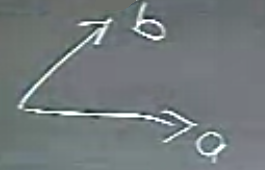
\includegraphics[height=2cm]{17_1.png}

Bu iki vektorden $q_1,q_2$ ortonormal vektorlerini cikartmak istiyorum. Ya
da, once ortogonal $A,B$, sonra ortonormal $q_1,q_2$ diyelim. Bunun icin once

\[ q_1 = \frac{ A}{||A||}, q_2 = \frac{ B}{||B||}  \]

Aslinda $a$'dan $A$ alinca, o vektorun isi bitmis kabul edilebilir. Bir yon
tamam, ama ilk yon oldugu icin onun ortogonal hali yeterli. Simdi ikinci
vektor nasil ortonormal olacak, cunku artik birinciye gore dik olmali, onu
oldugu gibi alamayiz. 

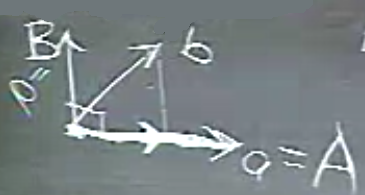
\includegraphics[height=2cm]{17_2.png}

Aradigimiz vektor $b$'nin $a$'ya yansimasi degil, ona tam dik olan
$e$. Eger $b$'nin formulu ``$b$'nin $a$'ya yansimasi, arti $e$'' ise, o
zaman ters yone gitmek icin cikartma islemini kullaniriz,

\[ B = b - [yansima] \]

$b$'nin $a$'ya yansimasi nedir? Yerine koyalim,

\[ B = b - \frac{ A^Tb}{A^TA}A \]

Bu formul dogru mu? Kontrol edelim, eger $B$ hakikaten $A$'ya ortogonal bir
vektor veriyorsa, o zaman $A^T$ ile carpilinca sifir elde etmeliyiz. 

\[ A^TB = A^T(b - \frac{ A^Tb}{A^TA}A) \]

\[ = A^Tb - \frac{ A^Tb}{A^TA}A^TA \]

\[ = A^Tb - A^Tb = 0 \]

Peki ya iki degil uc tane vektor olsaydi? Yani $A,B$'ye ek olarak bir de
$C$ hesaplamamiz gerekiyor. 

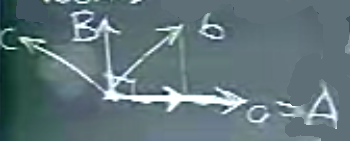
\includegraphics[height=2cm]{17_3.png}

Bu hesaba su sekilde bakabiliriz, aynen $B$'yi bulmak icin $b$'den $a$
yonunde olan yansimasinin kismini cikarttigimiz gibi, $C$'yi bulmak icin
$c$'den $a$ ve $b$ yonunde olan yansimasini kisimlari cikartmayi
dusunebiliriz.

\[ C = c - \frac{ A^Tc}{A^TA}A - \frac{ B^Tc}{B^TB}B \]

Yani $C \perp A$, $C \perp B$. 

Ornek

\[ 
a = 
\left[\begin{array}{r}
1 \\ 1 \\ 1
\end{array}\right],
b = 
\left[\begin{array}{r}
1 \\ 0 \\ 2
\end{array}\right]
 \]

Hemen $A = a$ deriz. $B$ nedir?

\[ 
B = 
\underbrace{
\left[\begin{array}{r}
1 \\ 0 \\ 2
\end{array}\right]}_{b}
-
\frac{ 3}{3}
\underbrace{
\left[\begin{array}{r}
1 \\ 1 \\ 1
\end{array}\right]}_{A}
=
\left[\begin{array}{r}
0 \\ -1 \\ 1
\end{array}\right]
 \]

$Q$'yu olusturalim. Unutmayalim, her $q$ birim vektor, normalize
olmali. Problem degil, degerleri ustten alirken her elemani uzunluguna
boleriz, 

\[ Q =
\left[\begin{array}{rrr}
\uparrow &  & \uparrow \\
q_1 & ... &  q_n \\
\downarrow &  & \downarrow 
\end{array}\right]
=
\left[\begin{array}{rr}
1/\sqrt{3} & 0 \\
1/\sqrt{3} & -1/\sqrt{2} \\
1/\sqrt{3} & 1/\sqrt{2} 
\end{array}\right]
 \]

Hatirlarsak ilk halimiz

\[ A =
\left[\begin{array}{rr}
1 & 1 \\
1 & 0\\
1 & 2
\end{array}\right]
 \]

seklindeydi. 

$Q$'nun kolon uzayi ile $A$'nin kolon uzayi arasindaki baglanti, fark
nedir? Kolon uzayi bir matrisin kolonlarinin tum kombinasyonlari ise, 3
boyutlu uzayda iki kolonum var, demek ki kolon uzayi bir duzlem (plane),
her iki matris icin durum bu. Alaka nerede? Iki duzlem de ayni! Tek
yaptigim ayni uzayi yaratan ama birbirine dik iki yeni vektor yaratmak
oldu. $Q$ vektorlerunden daha memnunum cunku $Q$ ortonormal. 

Peki Gram-Schmidt'i Lineer Cebir dilinde nasil daha temiz sekilde
gosteririm? Eliminasyon mesela 

\[ A = LU \]

olarak gosterilir. Gram-Schmidt'in karsiligi nedir? Sudur:

\[ A = QR \]


\[ 
\left[\begin{array}{rrr}
\uparrow &  \uparrow \\
a_1 &  a_2 \\
\downarrow &  \downarrow 
\end{array}\right]
=
\left[\begin{array}{rrr}
\uparrow &  \uparrow \\
q_1 &  q_2 \\
\downarrow &  \downarrow 
\end{array}\right]
\left[\begin{array}{rrr}
 &   \\
0 &  
\end{array}\right]
 \]

Yani $R$ ust ucgensel (lower triangular) bir matristir, sol alt kose
sifirdir. Niye? 

\[ 
=
\left[\begin{array}{rrr}
\uparrow &  \uparrow \\
q_1 &  q_2 \\
\downarrow &  \downarrow 
\end{array}\right]
\left[\begin{array}{rrr}
a_1^Tq_1 &  * \\
a_1^Tq_2 &  *
\end{array}\right]
 \]

Sifir $a_1^Tq_1$'dan geliyor. Ozetlemek gerekirse, $A$'yi alip $Q$'yu elde
ediyoruz, ve bu iki matris arasindaki iliski ust ucgensel olan $R$
matrisi. 

Gram-Schmidt Python kodu altta bulunabilir.

\begin{minted}{python}
import numpy.linalg as lin

A = np.array([[3., 4.],[5., 6.]])
m,n = A.shape
R = np.zeros((m,n))
Q = np.zeros((m,n))

for j in range(n):
    v = A[:,j]
    for i in range(j):
        R[i,j] = np.dot(Q[:,i].T,A[:,j])
        v=v-np.dot(R[i,j],Q[:,i])
    R[j,j] = lin.norm(v)
    Q[:,j] = v/R[j,j]
print Q, R
\end{minted}

\begin{verbatim}
[[ 0.51449576  0.85749293]
 [ 0.85749293 -0.51449576]] [[ 5.83095189  7.20294058]
 [ 0.          0.34299717]]
\end{verbatim}




\end{document}
